
\section*{5. Results Summary}
\subsection*{NOT Gate}
\begin{figure}[H] % [H] 強制圖片固定在文字當前的段落位置
    \centering
    % 左邊：圖片區塊
    \begin{minipage}[t]{0.48\textwidth}
        \vspace{0pt} % 修正頂部對齊基準點
        \centering
        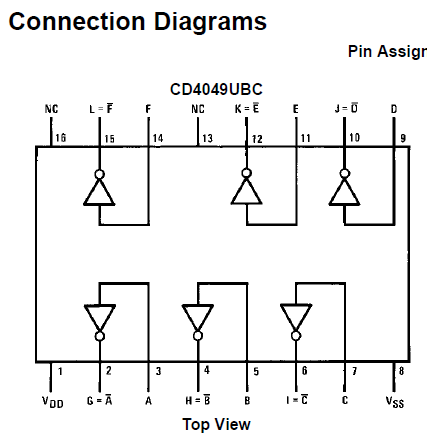
\includegraphics[width=\linewidth]{pic/not gate.png} % 請換成您的圖片檔名
        \captionof{figure}{not gate}
        \label{fig:not_image}
    \end{minipage}
    \hfill % 自動填滿中間間距
    % 右邊：文字區塊
    \begin{minipage}[t]{0.48\textwidth}
        \vspace{0pt} % 修正頂部對齊基準點
        \begin{table}[H]
        \centering
        \begin{tabularx}{0.7\textwidth}{>{\centering\arraybackslash}X | >{\centering\arraybackslash}X | >{\centering\arraybackslash}X}
\toprule
\textbf{Input (A)} & \textbf{O/P (0/1)} & \textbf{O/P (V)} \\
\hline
0 & & \\
1 & & \\
\bottomrule
\end{tabularx}
\end{table}
    \end{minipage}
\end{figure}

\hfill
\subsection*{AND Gate}
\noindent
\begin{figure}[H]
  \centering

   \begin{minipage}[t]{0.48\textwidth}
        \vspace{0pt} % 修正頂部對齊基準點
        \centering
        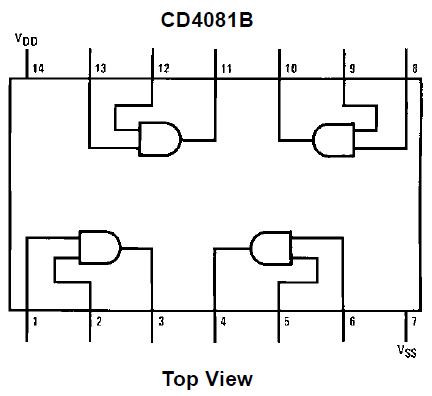
\includegraphics[width=\linewidth]{pic/and gate.png} % 請換成您的圖片檔名
        \captionof{figure}{not gate}
        \label{fig:and_image}
    \end{minipage}
\hfill % 自動填滿中間間距
\begin{minipage}[t]{0.48\textwidth}
  \begin{table}[H]
  \centering
  \small
  \begin{tabularx}{\linewidth}{c c | >{\centering\arraybackslash}X | >{\centering\arraybackslash}X}
  \toprule
  \textbf{In A} & \textbf{In B} & \textbf{O/P (0/1)} & \textbf{O/P (V)} \\
  \hline
  0 & 0 & & \\
  0 & 1 & & \\
  1 & 0 & & \\
  1 & 1 & & \\
  \bottomrule
  \end{tabularx}
  \end{table}
\end{minipage}
\end{figure}
\hfill

\subsection*{AND Gate}
\noindent
\begin{figure}[H]
  \centering

   \begin{minipage}[t]{0.48\textwidth}
        \vspace{0pt} % 修正頂部對齊基準點
        \centering
        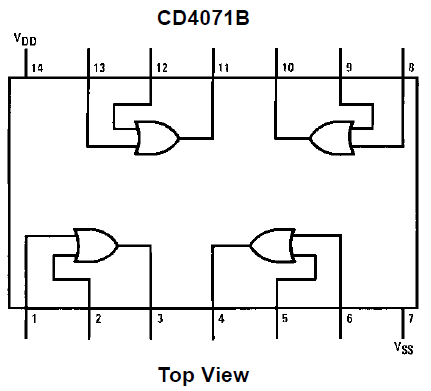
\includegraphics[width=\linewidth]{pic/or gate.png} % 請換成您的圖片檔名
        \captionof{figure}{not gate}
        \label{fig:or_image}
    \end{minipage}
\begin{minipage}[t]{0.48\textwidth}
  \begin{table}[H]
  \centering
  \small
  \begin{tabularx}{\linewidth}{c c | >{\centering\arraybackslash}X | >{\centering\arraybackslash}X}
  \toprule
  \textbf{In A} & \textbf{In B} & \textbf{O/P (0/1)} & \textbf{O/P (V)} \\
  \hline
  0 & 0 & & \\
  0 & 1 & & \\
  1 & 0 & & \\
  1 & 1 & & \\
  \bottomrule
  \end{tabularx}
  \end{table}
\end{minipage}
\end{figure}

\vspace{1.5em}